% !TeX root = ../../book.tex
\section{案例研讨}

\subsection{构建更大的立方体}

为了引出数学归纳法的整体方法,让我们看一道几何题并一起解决它。这个例子是精心挑选出来的,旨在说明当问题具有特定类型的结构时,数学归纳法如何与之关联;具体来说就是,某些真理、事实或洞察\emph{取决于}、\emph{依赖于}或可以从``先前的''事实\emph{推导}得出。这种对先前案例(或多个案例)的依赖使得过程具有\emph{归纳性},当我们观察到这种现象时,应用\emph{归纳法}几乎总是一个好主意。

\subsubsection*{$1$ 阶立方体到 $2$ 阶立方体}

让我们来考察一下立方数,尤其是,让我们试着用前一个立方数来描述一个立方数。想象一个 $1 \times 1 \times 1$ 的立方体,让它作为单位块。我们如何通过添加 $1 \times 1 \times 1$ 的块来构建尺寸为 $2 \times 2 \times 2$ 的``下一个最大''立方体?我们需要添加多少个?从算术上讲,我们知道答案:$2^3 = 8$ 且 $1^3 = 1$,因此我们需要添加 $7$ 个块才能得到正确的体积。好吧,这是一个具体的答案,但它并没有完全告诉我们如何排列这 $7$ 个块来构成一个立方体,也没有让我们深入了解如何回答构建\emph{更大}立方体这个问题。最终,我们想回答的是,需要多少块才能从 $100 \times 100 \times 100$ 的立方体构建出 $101 \times 101 \times 101$ 的立方体,而无需执行大量繁琐的计算;也就是说,我们希望最终找到问题的答案:给定一个 $n \times n \times n$ 的立方体,我们需要添加多少块才能将其构建为 $(n+ 1) \times (n+ 1) \times (n+ 1)$ 的立方体?考虑到这一点,让我们仔细思考这个最初的案例,并尝试用一般性的论点来回答它。

给定一个单位块,并且我们知道必须向其添加 $7$ 个块,让我们试着确定这 $7$ 个块应该放置在哪里,以形成 $2 \times 2 \times 2$ 的立方体。(为了简单起见,对于 $n$ 的任意值,我们把大小为 $n \times n \times n$ 的立方体称为 $n$ 阶立方体。在这个例子中,$n$ 的值只取自然数,即非负整数。)查看下面 $1$ 阶立方体和 $2$ 阶立方体的图片,并试着解释如何从一个立方体构建另一个立方体。

\begin{center}
    \begin{tikzpicture}
        \pic {annotated cuboid};

        \foreach \x in {0,1}
            \foreach \y in {0,1}
                \foreach \z in {0,1}
                    \pic [fill=white] at (4+\x,\y,\z) {annotated cuboid};
        % \pic [very thick,densely dashed,draw=blue] at (5,0) {annotated cuboid={width=30, height=5, depth=10, opacity=0.2}};
    \end{tikzpicture}
\end{center}

这是我们想要使用的一个合理的解释,因为它能指导我们给出从 $n$ 阶立方体构建 $(n+1)$ 阶立方体的一般解释,并且它是一种数学上优雅且简单的解释。从上面的 $1$ 阶立方体开始,将 $3$ 个暴露的面``放大''适当的量,在本例中为 $1$ 块。到目前为止,这占 $7$ 个块中的 $3$ 个:$2^3 = 1^3+3+\underline{\qquad}$。现在还缺哪里?

\begin{center}
    \begin{tikzpicture}
        \pic {annotated cuboid};
        \pic at (1,-1,0) {annotated cuboid};
        \pic at (0,-1,1) {annotated cuboid};
    \end{tikzpicture}
\end{center}

我们刚刚添加的块在每对块之间都产生了``间隙'',并且每个``间隙''都可以用一个块填充。这占了 $7$ 个块中的 $3$ 个:$2^3 = 1^3+3+3+\underline{\qquad}$。接下来呢?

\begin{center}
    \begin{tikzpicture}
        \pic {annotated cuboid};
        \foreach \x in {0,1}
            \foreach \y in {0,1}
                    \pic [fill=white] at (\x,\y,0) {annotated cuboid};
        \pic [fill=white] at (0,0,1) {annotated cuboid};
        \pic [fill=white] at (0,1,1) {annotated cuboid};
        \pic [fill=white] at (1,0,1) {annotated cuboid};
        % \pic [very thick,densely dashed,draw=blue] at (5,0) {annotated cuboid={width=30, height=5, depth=10, opacity=0.2}};
    \end{tikzpicture}
\end{center}

只剩下一个块需要填充,位于最顶角。添加这个块就完成了 $2$ 阶立方体的构建,并且我们还得到了如何使用以下图形和方程以数学的方式描述我们的构建过程:

\begin{center}
    \begin{tikzpicture}
        \pic {annotated cuboid};

        \pic [densely dashed] at (3, 0) {annotated cuboid};
        \pic [very thick,draw=blue] at (4.2,0,0) {annotated cuboid};
        \pic [very thick,draw=blue] at (3,1.2,0) {annotated cuboid};
        \pic [very thick,draw=blue] at (3,0,1.4) {annotated cuboid};

        \pic [densely dashed] at (7.5,1,0) {annotated cuboid};
        \pic [densely dashed] at (8.5,0,0) {annotated cuboid};
        \pic [densely dashed] at (7.5,0,1) {annotated cuboid};
        \pic [very thick,draw=red] at (8.7,1.2,-0.1) {annotated cuboid};
        \pic [very thick,draw=red] at (7.3,1,1.4) {annotated cuboid};
        \pic [very thick,draw=red] at (8.7,-0.2,1) {annotated cuboid};

        \foreach \x in {0,1}
            \foreach \y in {0,1}
                \pic [densely dashed, fill=white] at (12+\x,\y,0) {annotated cuboid};
        \pic [densely dashed, fill=white] at (12,0,1) {annotated cuboid};
        \pic [densely dashed, fill=white] at (12,1,1) {annotated cuboid};
        \pic [densely dashed, fill=white] at (13,0,1) {annotated cuboid};
        \pic [very thick,draw=olivegreen] at (13.3,1,1.4) {annotated cuboid};
    \end{tikzpicture}
\end{center}

\begin{center}
    \large $2^3 = 1^3+\textcolor{blue}{3}+\textcolor{red}{3}+\textcolor{olivegreen}{1}$
\end{center}

\subsubsection*{$2$ 阶立方体到 $3$ 阶立方体}

现在我们可能对如何描述这个过程有了更好的了解,但让我们多考察两个案例,以确保我们有完整的想法。

让我们从 $2$ 阶立方体开始,构造一个 $3$ 阶立方体。(如果碰巧你手上有各种尺寸的魔方,你甚至可以手动尝试一下!)我们可以遵循与上一个案例类似的步骤,只需适当更改数字即可。从相似的图形开始

\begin{center}
    \begin{tikzpicture}[scale=1]
        \pic {annotated cuboid};
        \foreach \x in {0,1}
            \foreach \y in {0,1}
                \foreach \z in {0,1}
                    \pic [fill=white] at (\x,\y,\z) {annotated cuboid};
        \foreach \x in {0,1,2}
            \foreach \y in {0,1,2}
                \foreach \z in {0,1,2}
                    \pic [fill=white] at (\x+4,\y,\z) {annotated cuboid};
    \end{tikzpicture}
\end{center}

可见我们需要``放大'' $2$ 阶立方体的三个暴露面,但在这种情况下,我们需要放大的量与以前($1$ 阶立方体)\emph{不同},因为我们现在使用的是更大的初始立方体。具体来说,每个面必须放大 $2 \times 2$ 的\emph{正方形}块(而在之前的情况下,我们添加了 $1 \times 1$ 的正方形块)因此,此添加过程的方程是
\[3^2 = 2^3+3\cdot2^2+\underline{\qquad}\]

\begin{center}
    \begin{tikzpicture}[scale=1]
        \foreach \x in {0,1}
            \foreach \y in {0,1}
                \pic [fill=white] at (\x,\y,2) {annotated cuboid};
        \foreach \x in {0,1}
            \foreach \z in {0,1}
                \pic [fill=white] at (\x,2,\z) {annotated cuboid};
        \foreach \y in {0,1}
            \foreach \z in {0,1}
                \pic [fill=white] at (2,\y,\z) {annotated cuboid};
    \end{tikzpicture}
\end{center}

这样做之后,我们发现需要使用 $2 \times 1$ 的块来填充这些放大的面之间的间隙(而在之前的情况下,我们添加了 $1 \times 1$ 的块)。到目前为止,添加过程的方程是
\[3^2 = 2^3+3\cdot2^2+3\cdot2+\underline{\qquad}\]

\begin{center}
    \begin{tikzpicture}[scale=1]
        \foreach \x in {0,1,2}
            \foreach \y in {0,1,2}
                \foreach \z in {0,1}
                    \pic [fill=white] at (\x,\y,\z) {annotated cuboid};
        \foreach \x in {0,1}
            \foreach \y in {0,1,2}
                \pic [fill=white] at (\x,\y,2) {annotated cuboid};
        \foreach \y in {0,1}
            \pic [fill=white] at (2,\y,2) {annotated cuboid};
    \end{tikzpicture}
\end{center}

这样做之后,我们看到只剩下顶角需要填充。因此,我们可以描述我们的构建过程及其相应的方程:

\begin{center}
    \begin{tikzpicture}[scale=1]
        \foreach \x in {0,1}
            \foreach \y in {0,1}
                \foreach \z in {0,1}
                    \pic [very thick, fill=white] at (\x,\y,\z) {annotated cuboid};

        \foreach \x in {0,1}
            \foreach \y in {0,1}
                \foreach \z in {0,1}
                    \pic [densely dashed, fill=white] at (\x+6,\y,\z) {annotated cuboid};
        \foreach \x in {0,1}
            \foreach \y in {0,1}
                \pic [very thick,fill=white,draw=blue] at (\x+6,\y,2.4) {annotated cuboid};
        \foreach \x in {0,1}
            \foreach \z in {0,1}
                \pic [very thick,fill=white,draw=blue] at (\x+6,2.3,\z) {annotated cuboid};
        \foreach \y in {0,1}
            \foreach \z in {0,1}
                \pic [very thick,fill=white,draw=blue] at (8.3,\y,\z) {annotated cuboid};

        \foreach \x in {0,1}
            \foreach \y in {0,1}
                \pic [densely dashed,fill=white] at (\x,\y-5,2) {annotated cuboid};
        \foreach \x in {0,1}
            \foreach \z in {0,1}
                \pic [densely dashed,fill=white] at (\x,-3,\z) {annotated cuboid};
        \foreach \y in {0,1}
            \foreach \z in {0,1}
                \pic [densely dashed,fill=white] at (2,\y-5,\z) {annotated cuboid};
        \foreach \x in {0,1}
            \pic [very thick,draw=red,fill=white] at (\x-0.3,-3,2.4) {annotated cuboid};
        \foreach \y in {0,1}
            \pic [very thick,draw=red,fill=white] at (2.3,\y-5,2.4) {annotated cuboid};
        \foreach \z in {0,1}
            \pic [very thick,draw=red,fill=white] at (2.3,-3,\z-0.4) {annotated cuboid};

        \foreach \x in {0,1,2}
            \foreach \y in {0,1,2}
                \foreach \z in {0,1}
                    \pic [densely dashed,fill=white] at (\x+6,\y-5,\z) {annotated cuboid};
        \foreach \x in {0,1}
            \foreach \y in {0,1,2}
                \pic [densely dashed,fill=white] at (\x+6,\y-5,2) {annotated cuboid};
        \foreach \y in {0,1}
            \pic [densely dashed,fill=white] at (8,\y-5,2) {annotated cuboid};
        \pic [very thick,draw=olivegreen] at (8.3,-3,2.4) {annotated cuboid};
    \end{tikzpicture}
\end{center}

\begin{center}
    \large $3^3 = 2^3+\textcolor{blue}{3 \cdot 2^2}+\textcolor{red}{3 \cdot 2}+\textcolor{olivegreen}{1}$
\end{center}

\subsubsection*{$n$ 阶立方体到 $n+1$ 阶立方体}

你知道这个过程如何泛化吗?如果我们从 $n$ 阶立方体开始怎么办?我们如何构造一个 $(n + 1)$ 阶立方体?我们按照前两个案例中使用的相同步骤进行操作。首先,我们通过添加三个\emph{正方形}块来放大三个暴露面。每个正方形块有多大?我们希望每个正方形块的大小与暴露面的大小相同,因此它们是 $n \times n$ 的正方形块,每个面有 $n^2$ 个单位块:

\begin{center}
    \begin{tikzpicture}[scale=0.20]
        \pic [densely dashed] {annotated cuboid={width=30, height=30, depth=30}};
        \pic at (2,0,0) {annotated cuboid={width=2, height=30, depth=30}};
        \pic at (0,2,0) {annotated cuboid={width=30, height=2, depth=30}};
        \pic at (0,0,3.6) {annotated cuboid={width=30, height=30, depth=3}};
    \end{tikzpicture}
\end{center}

\[(n+1)^3 = n^3+3n^2+\underline{\qquad}\]

接下来,我们要用行块填充这些放大面之间的间隙。这些行有多长?它们都位于我们刚刚添加的正方形块的边缘,因此它们的大小均为 $n \times 1$,每个间隙有 $n$ 个块:

\begin{center}
    \begin{tikzpicture}[scale=0.20]
        \pic [densely dashed] {annotated cuboid={width=30, height=30, depth=30}};
        \pic [densely dashed,fill=white] at (1,0,0) {annotated cuboid={width=2, height=30, depth=30}};
        \pic [densely dashed,fill=white] at (0,1,0) {annotated cuboid={width=30, height=2, depth=30}};
        \pic [densely dashed,fill=white] at (0,0,1) {annotated cuboid={width=30, height=30, depth=3}};
        \pic at (1,2,3.6) {annotated cuboid={width=30, height=2, depth=3}};
        \pic at (2,1,3.6) {annotated cuboid={width=2, height=30, depth=3}};
        \pic at (2.2,2,2.25) {annotated cuboid={width=2, height=2, depth=30}};
    \end{tikzpicture}
\end{center}

\[(n+1)^3 = n^3+3n^2+3n+\underline{\qquad}\]

最后就只剩下顶角需要填充了!所以,

\[(n+1)^3 = n^3+3n^2+3n+1\]

``等一下!'' 你可能会说,``我们早就知道这个结果了。'' 某种程度上,是的;上面的等式是一个代数恒等式,我们也可以通过展开左侧的乘积再合并同类项轻松得到它:

\begin{align*}
    (n + 1)^3 &= (n + 1) \cdot (n + 1)^2\\
    &= (n + 1) \cdot (n^2 + 2n + 1)\\
    &= (n^3 + 2n^2 + n) + (n^2 + 2n + 1) \\
    &= n^3 + 3n^2 + 3n + 1
\end{align*}

那么我们真正取得了什么成果呢?其实,以几何和视觉方式推导出这个恒等式其背后的要点是,它展示了这个恒等式如何表示某种\emph{归纳}过程。我们试图解释如何从先前已知的``事实''(下一个最小立方数,$n^3$)推导出该``事实''(立方数,$(n + 1)^3$),并正确解释如何做到这一点。将此与我们研究奇数之和为完全平方数时使用的方法进行比较。我们对技术之和的观察也隐含了一个归纳过程,尽管我们当时没有这样描述,但我们鼓励你现在思考一下这个问题。回顾一下我们之前的讨论,并尝试通过查看正方形块来写出如何用 $n^2$ 来写出 $(n + 1)^2$。它看起来像``明显的''代数恒等式吗?(如果你雄心勃勃,想一想用 $n^4$ 来写出 $(n + 1)^4$ 会发生什么。这背后有任何几何直觉吗?更高次幂呢?)

这种方法的好处是,我们知道如何用更小的立方数(一直到 $1$)来描述一个立方数;也就是说,每当我们在表达式中看到立方数时,我们都知道如何用更小的立方数和一些剩余项来写出该值。此外,这些表达式和剩余项中的每一个都具有某种固有结构,取决于具体讨论的立方数。因此,通过我们上面导出的表达式迭代地替换任意立方数(例如 $(n + 1)^3$),持续进行下去直到无法再替换为止,应该会产生一个具有一定内在对称性的方程。这个想法最好通过实际行动来说明,所以让我们看看会发生什么。让我们从之前推导出的表达式开始,对于 $n$ 的某个任意值,

\[(n+1)^3 = n^3+3n^2+3n+1\]

接着我们就知道一个类似的表达

\[n^3 = (n-1)^3+3(n-1)^2+3(n-1)+1\]

当我们给出 $n^3$ 的上述表达式的一般论证时,我们证明了这个方程成立,因为这仅依赖于 $n \ge 1$ 的事实。我们可以遵循相同的逻辑步骤,在整个过程中将 $n$ 替换为 $n - 1$,并最终得到上面第二个表达式,也就是 $(n - 1)^3$ 的表达式。(对于 $n$ 的任意值,这种情况都会继续下去吗?思考一下。当 $n \le 0$ 时,我们的论证有意义吗?比如说,从不同的立方体构造 $(-2) \times (- 2) \times (-2)$ 的立方体,这在物理上有意义吗?)

因此,我们可以替换上面一行中的 $n^3$ 项

\begin{center}
    \begin{tabular}{rcccccccc}
        $(n+1)^3=$ &     & $\cancel{n^3}$ & $+$ &   $3n^2$   & $+$ &   $3n$   & $+$ & $1$\\
                   & $+$ & $(n-1)^3$      & $+$ & $3(n-1)^2$ & $+$ & $3(n-1)$ & $+$ & $1$\\
    \end{tabular}
\end{center}

这也是一个代数恒等式,但我们肯定不会轻易地想到通过展开左侧的乘积并合并同类项来写出这个恒等式。这里,我们一遍又一遍地利用结果的结构,并得到我们原本不会想到的新表达式。让我们继续这个替换过程,看看它会带我们去到哪里!接下来,我们将 $(n - 1)^3$ 替换为相应的表达式,并得到

\begin{center}
    \begin{tabular}{rcccccccc}
        $(n+1)^3=$ &     &                    &     &   $3n^2$   & $+$ &   $3n$   & $+$ & $1$\\
                   &     & $\cancel{(n-1)^3}$ & $+$ & $3(n-1)^2$ & $+$ & $3(n-1)$ & $+$ & $1$\\
                   & $+$ & $(n-2)^3$          & $+$ & $3(n-2)^2$ & $+$ & $3(n-2)$ & $+$ & $1$\\
    \end{tabular}
\end{center}

也许你已经看清最终会去到哪里?我们可以一遍又一遍地进行这个替换过程,上面式子的列数将不断增长,向我们表明这里发生了一些深刻的、数学上对称的事情。但这个过程在哪里终止呢?我们想要写出这个迭代过程的简洁版本,并能够解释出现的每一项,因此必须知道它在哪里结束。还记得我们研究立方数的第一步吗?我们弄清楚了如何得到 $2^3 = 1^3 + 3 + 3 + 1$。由于这是我们构建此归纳过程的\emph{第一步},因此它应该是我们向后构建的\emph{最后一步},据此,我们可以写出

\begin{center}
    \begin{tabular}{rcccccccc}
        $(n+1)^3=$ &     &       &     &   $3n^2$   & $+$ &   $3n$   & $+$ & $1$\\
                   &     &       & $+$ & $3(n-1)^2$ & $+$ & $3(n-1)$ & $+$ & $1$\\
                   &     &       & $+$ & $3(n-2)^2$ & $+$ & $3(n-2)$ & $+$ & $1$\\
                   &     &       & $+$ & $3(n-3)^2$ & $+$ & $3(n-3)$ & $+$ & $1$\\
                   &     &       &     & $\vdots$   & $+$ & $\vdots$ & $+$ & $\vdots$\\
                   &     &       & $+$ & $3 \cdot 2^2$ & $+$ & $3 \cdot 2$ & $+$ & $1$\\
                   & $+$ & $1^3$ & $+$ & $3 \cdot 1^2$ & $+$ & $3 \cdot 1$ & $+$ & $1$\\
    \end{tabular}
\end{center}

这\emph{绝对}是我们做梦都想不到的恒等式!像这样的式子除了看起来比较漂亮之外,还可以让我们应用之前的知识,简化该表达式。为了了解如何做到这一点,让我们对上面的列应用求和符号,将一列同类项求和写成更简单的表达式:

\[(n+1)^3 = 1^3+3 \cdot \sum_{k=1}^{n}k^2+3 \cdot \sum_{k=1}^{n}k+\sum_{k=1}^{n}1\]

上一章中,我们通过几种不同的方法证明出

\[\sum_{k=1}^{n}k = \frac{n(n+1)}{2}\]

将该式应用于上面表达式最右边的两项,可以化简为

\[(n+1)^3 = 1^3+3 \cdot \sum_{k=1}^{n}k^2+\frac{3n(n+1)}{2}+n\]

这告诉我们什么?在所有这些代数运算之后,我们完成了什么?我们之前证明了前 $n$ 个自然数之和的结果,所以接下来自然要问:前 $n$ 个自然数的平方和是多少?我们如何回答这个问题呢?这是一个恶作剧问题,因为\emph{我们已经得到了}!让我们对上面的方程分离求和项再执行一两步代数步骤即可得到:

\begin{align*}
    (n+1)^3-1-n-\frac{3n(n+1)}{2} &= 3 \cdot \sum_{k=1}^{n}k^2 \\
    \frac{1}{3}(n+1)^3 - \frac{1}{3}(n+1) - \frac{n(n+1)}{2} &= \sum_{k=1}^{n}k^2
\end{align*}

这就是我们所完成的:我们推导出了前 $n$ 个自然数的平方和公式!当然,上面一行左边的表达式不是特别好看,我们可以进一步简化,你可以亲自验证一下是否会得到以下表达式:

\[\sum_{k=1}^{n}k^2 = \frac{1}{6}n(n+1)(2n+1) \]

\subsubsection*{``依此类推''并不严谨!}

基于所有这些工作,我们想指出一些``寓意''。第一个寓意是,归纳论证是发现新的、有趣的数学思想和结论的好方法。你有没有想过这个问题与奇数之和有什么关系?如果没有,我们强烈建议你现在就尝试一下,并思考将其进一步推广到四维或五维``立方体''。除了带给你其他有趣的结果之外,它对于学习抽象思维和应用归纳过程也具有难以置信的指导意义。第二个寓意更像是一种承认:我们还\emph{没有}从技术上\emph{证明}上面的前 $n$ 个自然数平方和的公式。看起来我们的推导是有效的,并得到了``正确答案'',但有一个明显的问题:省略号!

在展开 $(n + 1)^3$ 得到每列的求和项时,在这些列中间写出 $\vdots$ 有助于引导我们的直觉,但\emph{这在不是严谨的数学技术}。我们如何\emph{知道}中间所有项都符合我们的预期?我们如何确定所有立方体图形都能完美地转化为我们写下的数学表达式?``一直递降到 $1$''到底是什么意思?

举个例子,考虑下面的数字列表:
\[1,2,3,4,\dots 100\]
你可能将其解释为``$1$ 到 $100$ 之间的所有自然数(含 $1$ 和 $100$)''。这似乎很合理。但万一我们\emph{实际}指的是下面这个数列呢?
\[1, 2, 3, 4, 7, 10, 11, 12, 14, \dots , 100\]
为什么是这个数列?这当然有可能,我们指的是 $1$ 到 $100$ 的自然数中,英文拼写不含字母"i"的数字的列表。这不是很明显吗?

重点是:当与朋友交流并\emph{表达}一些想法时,写 $1,2,3, \dots, 100$ 没有问题,可以确保受众\emph{确切地}知道你的意思。但总的来说,我们不能假设读者会自然而然地凭直觉理解我们试图传达的内容;我们应该尽可能做到\emph{明确}和\emph{严谨}。

现在你可能会觉得我们在吹毛求疵,但更重要的一点是,有一种数学方法可以使这个论证更加\emph{精确},从而构成一个完全有效的\emph{证明}。到目前为止,我们所做的一切都有助于引导我们的直觉,但我们还需要做更多的工作来确保我们的论点完全令人信服。一般来说,要使此类论证变得严格,还需要一些其他概念,我们将在下一章中研究这些概念,然后再回到这个主题。然而,与此同时,让我们再看一个例子来练习这种直观的论证风格,并识别归纳法何时是一种适用的技术。

\subsection{平面上的线}

拿一张干净的纸、一支笔和一把尺子。这张纸上有多少个区域?只有一个,对吧?在纸上画一条直线。现在有两个区域。再画一条与第一条直线相交的直线。现在有多少个区域?数一数,总共有四个。绘制第三条直线线,与前两条直线相交,但不过前两条直线的交点。(也就是说,总共应该有三个交点。)现在有多少个区域?你能在不数的情况下预测答案吗?当有 $4$ 条直线时会怎样?$5$ 个呢?$100$ 个呢?我们如何解这道题并最终解决它?让我们给出一个更正式的陈述,以确保我们用同样的方式思考:

考虑无限平面(二维表面)上的 $n$ 条直线,互不\emph{平行}且没有两条以上的线过\emph{同一交点}。这些直线分割出多少个不同区域?

当 $n$ 很小时(例如,$n$ 不超过 $5$),我们可以手工画一些例子,让这些例子来引导我们的直觉,对\emph{任意} $n$ 值进行一般论证。(请注意,此策略与我们在上一题中所做的非常相似:识别较小案例的模式,识别这些案例中可以泛化的相关部分,然后抽象为任意案例。)具体来说,我们想尝试确定一幅图中的区域数量如何\emph{取决于}线条较少的图中的区域数量。当我们画一条新的直线时会发生什么?我们能否确定它是如何改变现有区域的?我们能以某种方式计算一下它创建了多少个区域吗?在继续阅读之前,请自行对本题进行一些调研。如果你得出一些结果,请将你的工作与我们下面遵循的步骤进行比较。 

让我们从 $n = 2$ 开始。我们知道一条直线将平面分为 $2$ 个区域;当我们添加第二条直线时会发生什么?我们知道会有 $4$ 个区域,因为我们可以画出图形并数出这些区域:

\begin{center}
    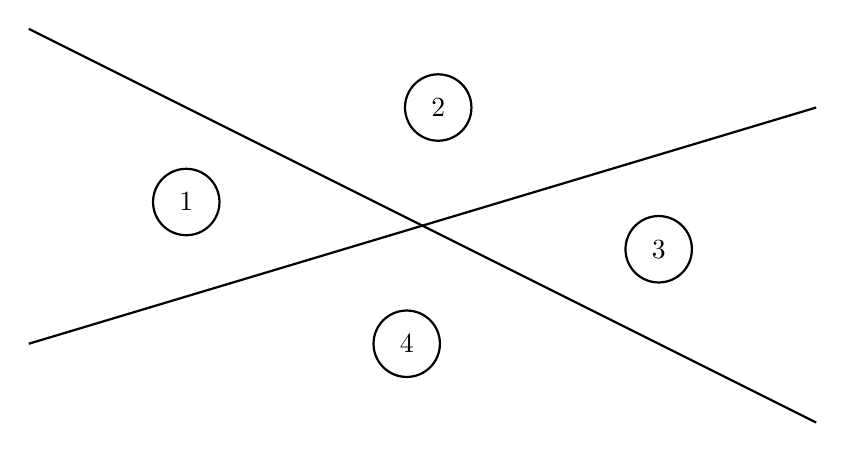
\begin{tikzpicture}[thick]
        \draw (-5,2.5) -- (5,-2.5);
        \draw (-5,-1.5) -- (5,1.5);
        \node[draw,circle,minimum size=24pt,inner sep=0,anchor=center] at (-0.2,-1.5) {$4$};
        \node[draw,circle,minimum size=24pt,inner sep=0,anchor=center] at (3,-0.3) {$3$};
        \node[draw,circle,minimum size=24pt,inner sep=0,anchor=center] at (-3,0.3) {$1$};
        \node[draw,circle,minimum size=24pt,inner sep=0,anchor=center] at (0.2,1.5) {$2$};
    \end{tikzpicture}
\end{center}

然而,这只是两条直线相交的一种\emph{具体情况}。我们怎么知道无论我们如何画这两条线,\emph{总能}得到四个区域?也就是说,我们能否以某种方式结合直线数量 $n = 2$ 这一事实来描述这是\text{如何}发生的?思考一下!

下面是我们的方法。请注意,当我们添加第二条直线时,每个已经存在的区域都会被分成两部分,并且\emph{无论你如何绘制直线},只要我们确保两条直线不平行,结果都是这样。也就是说,如果我们用一条直线将平面分成两个区域,

\begin{center}
    \begin{tikzpicture}[thick]
        \draw (-5,2.5) -- (5,-2.5);
        \node[draw,circle,minimum size=24pt,inner sep=0,anchor=center] at (-3,0.3) {$1$};
        \node[draw,circle,minimum size=24pt,inner sep=0,anchor=center] at (0.2,1.5) {$2$};
    \end{tikzpicture}
\end{center}

然后添加一条新的直线会将每个现有区域分成两部分。这会向整个平面添加两个新的区域,总共四个区域:

\begin{center}
    \begin{tikzpicture}[thick]
        \draw (-5,2.5) -- (5,-2.5);
        \draw [color=red] (-5,-1.5) -- (0,0)  node[midway,below,sloped]{分割区域 1}
        -- (5,1.5) node[midway,above,sloped]{分割区域 2} ;
        \node[draw,circle,minimum size=24pt,inner sep=0,anchor=center,color=red] at (-0.2,-1.5) {$4$};
        \node[draw,circle,minimum size=24pt,inner sep=0,anchor=center,color=red] at (3,-0.3) {$3$};
        \node[draw,circle,minimum size=24pt,inner sep=0,anchor=center] at (-3,0.3) {$1$};
        \node[draw,circle,minimum size=24pt,inner sep=0,anchor=center] at (0.2,1.5) {$2$};
    \end{tikzpicture}
\end{center}

当 $n = 3$ 时呢?在这种情况下,我们需要考虑向具有两条直线和四个区域的图形中添加第三条直线。我们想要提出一个不依赖于线的特定排列的论证,因此我们最终唯一能用的事实是线之间互不平行,且任何交点仅位于两条线(而不是三条或更多)上。不过,就目前而言,查看特定的线条排列会有所帮助,以便我们讨论相同的图形;我们可以利用对这个特定图形的观察来指导我们的一般论证。让我们从下方具有两条直线的图开始,向其中添加第三条线,我们让第三条线的交点都在初始交点``附近''或在图的范围内,这样我们就缩放图形了:

\begin{center}
    \begin{tikzpicture}[thick]
        \draw (-5,2.5) -- (5,-2.5);
        \draw (-5,-1.5) -- (5,1.5);
        \draw [color=red] (-5,1) -- (-1.8085,0.9043) node[midway,below,sloped]{\small 分割区域 1} 
        -- (2.5758,0.7727) node[midway,above,sloped]{\small 分割区域 2}
        -- (5,0.7) node[midway,below,sloped]{\small 分割区域 3};
        \node[draw,circle,minimum size=16pt,inner sep=0,anchor=center] at (-0.2,-1.5) {$4$};
        \node[draw,circle,minimum size=16pt,inner sep=0,anchor=center] at (3,-0.3) {$3$};
        \node[draw,circle,minimum size=16pt,inner sep=0,anchor=center] at (-3,-0.3) {$1$};
        \node[draw,circle,minimum size=16pt,inner sep=0,anchor=center] at (0.2,2) {$2$};
        \node[draw,circle,minimum size=16pt,inner sep=0,anchor=center,color=red] at (-4,1.45) {$5$};
        \node[draw,circle,minimum size=16pt,inner sep=0,anchor=center,color=red] at (0.1,0.45) {$6$};
        \node[draw,circle,minimum size=16pt,inner sep=0,anchor=center,color=red] at (4.61,1.05) {$7$};
    \end{tikzpicture}
\end{center}

很明显现在我们有 $7$ 个区域。我们将第三条线设置为不同的颜色,以便我们可以识别``新''区域出现的位置:一个区域(下方区域,区域 $4$)保持不变,但其他三个区域被一分为二,每个``分割''都会让我们的计数加 $1$(原来有 $1$ 个区域,现在有 $2$ 个)。如果我们以不同的方式绘制这条直线会怎样?

\begin{center}
    \begin{tikzpicture}[thick]
        \draw (-5,2.5) -- (5,-2.5);
        \draw (-5,-1.5) -- (5,1.5);
        \draw [color=red] (0,2.5) -- (-0.8333,0.4167) node[midway,right,sloped,rotate=-90]{\small 分割区域 2} 
        -- (-1.1364,-0.341) node[midway,left,sloped,rotate=-90]{\small 分割区域 1}
        -- (-2,-2.5) node[midway,right,sloped,rotate=-90]{\small 分割区域 4}; 
        \node[draw,circle,minimum size=16pt,inner sep=0,anchor=center] at (-0.2,-1) {$4$};
        \node[draw,circle,minimum size=16pt,inner sep=0,anchor=center] at (3,-0.3) {$3$};
        \node[draw,circle,minimum size=16pt,inner sep=0,anchor=center] at (-3,-0.3) {$1$};
        \node[draw,circle,minimum size=16pt,inner sep=0,anchor=center] at (1,2) {$2$};
        \node[draw,circle,minimum size=12pt,inner sep=0,anchor=center,color=red] at (-0.7,0.05) {$5$};
        \node[draw,circle,minimum size=16pt,inner sep=0,anchor=center,color=red] at (-1.5,1.8) {$6$};
        \node[draw,circle,minimum size=16pt,inner sep=0,anchor=center,color=red] at (-2.5,-1.4) {$7$};
    \end{tikzpicture}
\end{center}

同样的现象再次发生,其中一个区域保持不变,但其他三个区域一分为二。(我们怎么知道没有任何其他区域未绘制在我们这个比例的图形内?这并不像看上去的那么容易回答,值得深刻考虑。)尝试三条线的其他排列方式,并试图说服自己这种情况总会发生;此外,思考一下\emph{为什么}会出现这种情况,以及我们\emph{如何}解释这种情况一定会发生。不过,在给出一般性解释之前,我们先来看另一个小案例。

当 $n = 4$ 时,我们从 $3$ 条直线和 $7$ 个区域的平面开始,然后添加第四条直线,该线不与任何现有线平行,并且不穿过任何现有交点。同样,我们想要提出一个与特定的线条排列无关的论证,但是查看下面的具体图形将有助于引导我们的直觉来提出该论证:

\begin{center}
    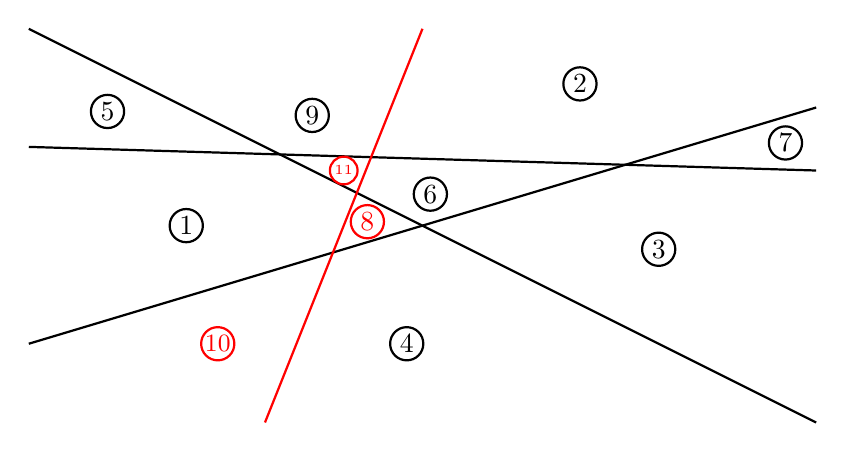
\begin{tikzpicture}[thick]
        \draw (-5,2.5) -- (5,-2.5);
        \draw (-5,-1.5) -- (5,1.5);
        \draw  (-5,1) -- (5,0.7);
        \draw [color=red] (0,2.5) -- (-2,-2.5);
        \node[draw,circle,minimum size=12pt,inner sep=0,anchor=center] at (-0.2,-1.5) {$4$};
        \node[draw,circle,minimum size=12pt,inner sep=0,anchor=center] at (3,-0.3) {$3$};
        \node[draw,circle,minimum size=12pt,inner sep=0,anchor=center] at (-3,0) {$1$};
        \node[draw,circle,minimum size=12pt,inner sep=0,anchor=center] at (2,1.8) {$2$};
        \node[draw,circle,minimum size=12pt,inner sep=0,anchor=center] at (-4,1.45) {$5$};
        \node[draw,circle,minimum size=12pt,inner sep=0,anchor=center] at (-1.4,1.4) {$9$};
        \node[draw,circle,minimum size=10pt,inner sep=0,anchor=center,color=red] at (-1,0.7) {\tiny $11$};
        \node[draw,circle,minimum size=12pt,inner sep=0,anchor=center] at (4.61,1.05) {$7$};
        \node[draw,circle,minimum size=12pt,inner sep=0,anchor=center,color=red] at (-0.7,0.05) {$8$};
        \node[draw,circle,minimum size=12pt,inner sep=0,anchor=center] at (0.1,0.4) {$6$};
        \node[draw,circle,minimum size=12pt,inner sep=0,anchor=center,color=red] at (-2.6,-1.5) {\small $10$};
    \end{tikzpicture}
\end{center}

请注意,三个原始区域保持不变(区域 $3$、区域 $5$ 和区域 $7$),其他四个区域一分为二。你注意到这里存在一个模式吗?似乎对于我们检查过的每个 $n$,添加第 $n$ 条线会使 $n-1$ 个区域保持不变,而其余区域则被一分为二。让我们尝试解释为什么会出现这种情况。请记住,当我们绘制 $n$ 条直线时,我们试图确定出现了多少个区域,因此让我们为该值分配一个``名称'',以便我们可以引用它;假设 $R(n)$ 表示在平面上绘制 $n$ 条直线所创建的区域数,且没有两条线平行,并且没有交点在两条以上的线上。在上面示例中,我们考虑了 $n$ 的较小取值,并研究了添加新的直线时会发生什么变化;也就是说,我们可以通过已知 $R(n - 1)$ 算出 $R(n)$ 的值。让我们整理一下我们的观察结果,以便它们适用于\emph{任意} $n$ 值。

假设我们已知 $R(n)$。(为什么我们可以这样做?对于某个特定的 $n$,我们是否确实知道 $R(n)$ 的特定值?这个值是什么?如何知道的?)假设我们在平面上有一个\emph{任意} $n$ 线图,满足上面题目陈述中给出的两个条件。这些直线创建了多少个区域?是的,正是 $R(n)$。现在,当我们添加第 $(n + 1)$ 条直线时会发生什么?关于这条线以及它如何改变图形,我们可以确定什么?其实,我们真正掌握的唯一信息是:

\begin{enumerate}[label=(\alph*)]
    \item 这条新的直线与现有的 $n$ 条直线中的任何一条都不平行;
    \item 这条新的直线不经过任何现有的交点。
\end{enumerate}

现在,条件 (a) 告诉我们这条新的直线必须与\emph{所有}现有的 $n$ 条直线线相交;平行线不相交,非平行线必然相交于某处。因此,我们必须在图上创建 $n$ 个新的交点。这些交点会与任何现有交点重合吗?不会!这正是条件 (b) 告诉我们的。这两条信息合在一起告诉我们,无论我们如何绘制这条新的直线,只要它满足题目的要求,这条直线上\emph{一定}会出现 $n$ 个``特殊''点。这些特殊点正是新线与现有线的交点。

我们现在想利用这些特殊点来识别图中的新区域。回顾一下我们上面研究的案例:识别新的交点,看看是否可以将它们与新的区域关联起来。也许用圆点标记这些交点并用 $\textbf{×}$ 标记新区域会有所帮助,让它们更容易辨认。我们在下面为你展示了一个示例,其中 $n = 4$。你注意到了什么?你能用这些点来帮助识别添加第 $n$ 条直线后创建了多少新区域吗?思考一下,然后继续阅读。

\begin{center}
    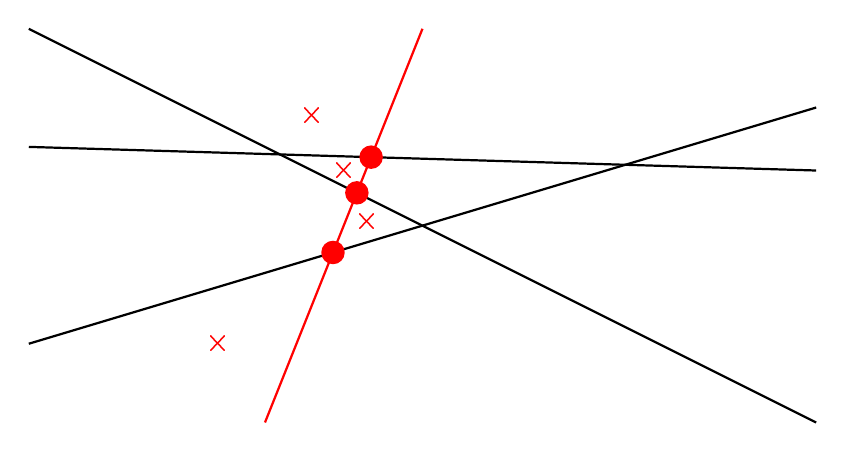
\begin{tikzpicture}[thick]
        \draw (-5,2.5) -- (5,-2.5);
        \draw (-5,-1.5) -- (5,1.5);
        \draw  (-5,1) -- (5,0.7);
        \draw [color=red] (0,2.5) -- (-2,-2.5);
        \node[minimum size=14pt,anchor=center,color=red,very thick] at (-1.4,1.4) {$\textbf{×}$};
        \node[minimum size=14pt,anchor=center,color=red,very thick] at (-1,0.7) {$\textbf{×}$};
        \node[minimum size=14pt,anchor=center,color=red,very thick] at (-0.7,0.05) {$\textbf{×}$};
        \node[minimum size=14pt,anchor=center,color=red,very thick] at (-2.6,-1.5) {$\textbf{×}$};
        \node[fill,circle,inner sep=3pt,color=red] at (-0.6522,0.8696) {};
        \node[fill,circle,inner sep=3pt,color=red] at (-0.8333,0.4167) {};
        \node[fill,circle,inner sep=3pt,color=red] at (-1.1364,-0.341) {};
    \end{tikzpicture}
\end{center}

没错!任意两个相邻新交点之间,都有一条\emph{线段}将一个区域一分为二!剩下的就是确定我们创建了多少个新的此类线段。由于每条线段都将唯一\emph{一个}现有区域一分为二,因此这将准确地告诉我们创建了多少个新区域。我们已知,第 $(n + 1)$ 条直线线创建了 $n$ 个新的交点。想想这些点是如何排列在直线上的。任意两个``连续''点都会创建一条线段,但极点也会创建无限线段(永远延申下去经过这些极点)。总共有多少个?正好是 $n + 1$。(参考上图,$n = 3$。我们看到有 $3$ 个新交点和 $4$ 条新线段,其中两个是无限射线。)这意味着有 $n + 1$ 条线段将区域一分为二,因此我们恰好创建了 $n + 1$ 个新区域!这让我们可以说
\[R(n + 1) = R(n) + n + 1\]
哇,多好的观察啊!我们花了一些时间研究示例并进行了一些几何论证,但最终我们做到了。我们已经确定了这个问题的一些归纳结构;我们发现一个情况如何依赖另一个情况。也就是说,我们发现了 $R(n+1)$ 如何依赖 $R(n)$。这还没有完全解决这个问题,但我们现在已经非常接近了。剩下的就是用类似的表达式替换 $R(n)$,并不断执行此操作,直到达到我们已知的 $R(1) = 2$。观察:

\begin{center}
    \begin{tabular}{rcccccccccc}
        $R(n+1)$ & $=$ &          & &            &     &            &     & $\cancel{R(n-1)}$ & $+$ & $n+1$\\
                 & $=$ &          & &                   &     & $\cancel{R(n-1)}$ & $+$ & $n$ & $+$ & $n+1$\\
                 & $=$ &          & & $\cancel{R(n-2)}$ & $+$ & $(n-1)$           & $+$ & $n$ & $+$ & $n+1$\\
                 & $\vdots$ &     & &  &  &  &  &  &  & \\
                 & $=$ &          & & $\cancel{R(2)}+3$ & $+$ & $\dots$ & $+$ & $n$ & $+$ & $n+1$ \\
                 & $=$ & $R(1)+2$ & $+$ & $3$               & $+$ & $\dots$ & $+$ & $n$ & $+$ & $n+1$ \\
    \end{tabular}
\end{center}

因为我们知道 $R(1) = 2$,所以我们可以说
\[R(n + 1) = 2 + \big(2 + 3 + \dots + n + (n + 1)\big) = 2 + \Bigg(\sum_{k=1}^{n+1}k\Bigg)-1 = 1+\sum_{k=1}^{n+1}k\]
而这正是我们之前研究过的求和公式!(另请注意,我们必须减去 $1$,因为括号中缺少求和的第一项。)回想一下 $\sum_{k=1}^{n} k = \frac{n(n+1)}{2}$,为了表示上面等式中的求和,我们只需将 $n$ 替换为 $n + 1$ 即可。因此,
\[R(n + 1) = 1+\frac{(n+1)(n+2)}{2}\]
我们要进行的最后一步简化是将整个方程中的 $n+1$ 替换为 $n$,因为使用 $R(n)$ 的表达式更有意义(对 $n$ 的值有什么要求?)
\[R(n + 1) = 1+\frac{n(n+1)}{2}\]
最终,我们找到了开头问题的答案!在这个过程中,我们采用了\emph{归纳}技术:我们解释了一个``事实''(即 $R(n + 1)$ 的值)如何\emph{取决于}``前一个事实''(即 $R(n)$ 的值),并使用这些迭代依赖关系进行反向运算,直到达到一个特定的\emph{已知}值,即 $R(1)$。

我们想再次指出,我们在本节中所做的推导和观察只是引导我们的直觉从而得出答案,并不是\emph{严格证明}。问题出在 ``$\dots$'' 身上,省略号不是具体的、``官方''的数学方法来捕获归纳技术背后的归纳过程。此外,我们解决``平面中的线''问题的方法是从 $n - 1$ 条线的图形\emph{开始,构建}一个包含 $n$ 条线的新图;这样可以吗?为什么这实际上告诉了我们有关 $n$ 条线的\emph{任意}图的信息?所有这些图都来自于少了一条线的较小图吗?

在接下来的两章中,我们将学习必要的工具来充分描述我们迄今为止所做事情的严格方法,在那之后的章节中,我们将使用这些工具让数学归纳法变得正式而严谨。不过,现在我们想给出归纳法的启发式定义,并继续研究依赖归纳技术的有趣问题和观察结果。练习这些类型的问题 --- 学习何时识别归纳过程、如何使用它、如何使用该结构来解决问题等等 --- 将在未来非常有帮助,我们不需要深入到数学技术细节。(至少,现在还不需要!)

\subsection{习题}

\subsubsection*{温故知新}

以口头或书面的形式简要回答以下问题。这些问题全都基于你刚刚阅读的内容,所以如果忘记了具体的定义、概念或示例,可以回去重读相关部分。确保在继续学习之前能够自信地回答这些问题,这将有助于你的理解和记忆!

\begin{enumerate}[label=(\arabic*)]
    \item 归纳过程有哪些特征?
    \item 我们如何证明 $\sum_{k=1}^{n}k = \frac{n(n+1)}{2}$ 是正确的?我们的方法是如何归纳的?(如果你不记得了,请重读第 \ref{sec:section1.4.2} 节!)
    \item 为什么我们可以把上一个问题中提到的求和公式,用 $n+1$ ``替换'' $n$,并且知道它仍然成立?我们也可以将 $n$ 替换为 $n - 1$ 吗?
    \item 通过代数步骤获得前 $n$ 个自然数平方和的最终表达式;也就是说,验证
    \[\frac{1}{3}(n+1)^3-\frac{1}{3}(n+1)-\frac{n(n+1)}{2} = \frac{1}{6}n(n+1)(2n+1)\]
    \item 试着回忆一下向平面中添加第 $(n+1)$ 条直线正好会创建 $n+1$ 个新区域的论点。你能为朋友证明这个论点并说服他/她它是有效的吗?
    \item 求前 $n$ 个自然数的平方和,为什么不能把前 $n$ 个自然数之和的公式平方呢?为什么这是错误的?
\end{enumerate}

\subsubsection*{小试牛刀}

尝试回答以下问题。这些题目要求你实际动笔写下答案,或(对朋友/同学)口头陈述答案。目的是帮助你练习使用新的概念、定义和符号。题目都比较简单,确保能够解决这些问题将对你大有帮助!

\begin{enumerate}[label=(\arabic*)]
    \item 在平面中画 $5$ 条直线(满足原题的两个条件)并验证是否有 $16$ 个区域。你还能验证 $6$ 条线产生 $22$ 个区域吗?
    \item 给出序列 $1, 2, 3, 4, \dots , 100$ 的另一种解释,而不仅仅是从 $1$ 到 $100$ 的所有自然数。(回想一下我们给出的例子:$1$ 到 $100$ 之间所有英文拼写中不含字母"i"的数字。)
    \item 提出一个将 $(n + 1)^4$ 与 $n^4$ 联系起来的代数表达式,就像我们对立方所做的那样。\\ 
    (\textbf{挑战题:}你能为刚刚推导出的表达式给出\emph{几何}解释吗?)
    \item \textbf{挑战题:}让我们将``平面上的线''这题提升一个维度!考虑三维空间中有 $n$ 个平面。会创建多少个区域?假设没有两个平面平行,并且没有三个或以上平面相交于一条直线。(想想这两个条件如何直接类比于``线''那题的给定条件。)
\end{enumerate}